\chapter[Metodologia]{Metodologia} \label{metodologia}

A metodologia deste trabalho está descrita nas próximas seções e está dividida em Ferramentas de Desenvolvimento e Metodologia de Desenvolvimento.

\section{Ferramentas de desenvolvimento}

  Para a realização do porte do jogo para \textit{Game Boy Advance}, são necessários dois ambientes principais: um ambiente de desenvolvimento onde seja possível implementar o jogo e exportar o binário executável para o console e um ambiente para testar o executável gerado, sendo esse físico ou emulado.

  \subsection{Ambiente de desenvolvimento}

    O jogo será reescrito utilizando a linguagem C++, na versão 11, pois provê uma série de recursos e estruturas não presentes na linguagem C que facilitarão o desenvolvimento do jogo.

    O ambiente de desenvolvimento utilizado para a implementação do jogo consiste do \textit{kit} de desenvolvimento devkitARM, ferramentas para manipulação das imagens e áudio do jogo.

    \subsubsection{\textit{devkitPro} e \textit{devkitARM}}

      O \texttt{\textbf{devkitPro}}\footnote{\textit{devkitPro}, disponível em \url{https://devkitpro.org/}} é uma organização que provê conjuntos de ferramentas para desenvolvimento de jogos em diversos consoles da \textit{Nintendo}, como \textit{Nintendo GBA}, \textit{Nintendo Wii}, \textit{Nintendo Switch}, dentre outros.

      Dentre esses conjuntos de ferramentas encontra-se o \textit{devkitARM}, \textit{toolchain} que contém o ambiente de desenvolvimento necessário para realizar a compilação do código escrito em C/C++ para a arquitetura de processadores ARM existente no GBA, citado na seção \ref{gba} do capítulo \ref{fundamentacao}.

    \subsubsection{Manipulação das imagens}

      Para o ajuste das imagens do jogo para a resolução de tela do GBA, foi utilizada a ferramenta de manipulação de imagens \textbf{GIMP}\footnote{GNU Image Manipulation Program, disponível em \url{https://www.gimp.org/}}, versão 2.8.

      Para realizar a conversão das imagens para um formato legível no GBA, foi utilizada uma biblioteca C chamada \textbf{GRIT}\footnote{\textit{GBA Raster Image Transmogrifier}, disponível em \url{http://www.coranac.com/projects/grit/}}.

    \subsubsection{Manipulação do áudio}
      Para a manipulação do áudio do jogo foram utlizadas três ferramentas: \texttt{\textbf{avconv}}\footnote{\texttt{avconv}, disponível em \url{https://github.com/libav/libav}} e \texttt{librosa}\footnote{\texttt{\textbf{librosa}}, disponível em \url{https://github.com/librosa/librosa}} para \textit{downsampling} das músicas; e \texttt{\textbf{modplug tracker}}\footnote{\textit{Open Modplug Tracker}, disponível em \url{http://openmpt.org/features}} para realizar a conversão das músicas para \texttt{.mod}.


  \subsection{Ambiente de teste}

    \subsubsection{Emulador}

      Para a realização de testes com os executáveis gerados pelo \textit{devkitARM} está sendo utilizado um emulador de \textit{Game Boy Advance}, chamado \textbf{\textit{VisualBoyAdvance-M}}\footnote{\textit{VisualBoyAdvance-M}, disponível em \url{https://github.com/visualboyadvance-m/visualboyadvance-m}}.

    \subsubsection{\textit{Console}} \label{console}

      O \textit {console} que está sendo utilizado como ambiente de testes real é um \textbf{\textit{Nintendo DS}}\footnote{\textit{Nintendo DS}, disponível em \url{https://www.nintendo.com/consumer/systems/selectds.jsp}}, que possui um \textit{slot} para cartuchos de \textit{Game Boy Advance}. Neste trabalho está sendo utilizado um cartucho especial onde é possível escrever arquivos executáveis diretamente nele.

      Para a escrita dos arquivos executáveis neste cartucho é utilizado o dispositivo \textbf{\textit{EZFlash II}}\footnote{\textit{EZ Flash II}, disponível em \url{http://www.ezfadvance.com/cards/EZ-Flash_2.htm}}. Como essa é uma versão antiga do produto, é necessário instalar um cliente para \textit{upload} dos arquivos para o cartucho. Este cliente só possui compatibilidade com \textit{\textbf{Windows XP}}\footnote{\textit{Windows XP}, disponível em \url{https://support.microsoft.com/pt-br/help/14223/windows-xp-end-of-support}}, fazendo com que seja necessário instalar uma máquina virtual com o sistema operacional.

\section{Metodologia de desenvolvimento}

  \subsection{Desenvolvimento da \textit{Engine}}

    Para contribuir com uma arquitetura mais manutenível, foi optado por desacoplar a \textit{engine} do jogo em si. A \textit{engine} ficará responsável por implementar os módulos genéricos do jogo, enquanto que o jogo em si conterá as funcionalidades mais específicas.

    A \textit{engine} conterá uma classe que irá representar um objeto do jogo (do inglês, \textit{game object}). Esta classe ficará responsável por conter o comportamento genérico de um objeto dentro do jogo (podendo este ser um personagem, uma plataforma, um item coletável, etc.). Ele será representado da seguinte maneira:

    \vspace{\onelineskip}

    \begin{figure}[H]
      \centering 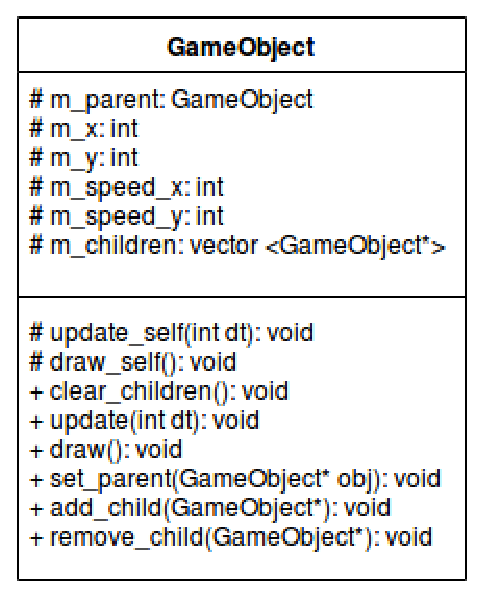
\includegraphics[keepaspectratio=true,scale=0.6]{figuras/game-object.eps}
      \caption[Modelagem inicial da classe \textit{GameObject}]
        {Modelagem inicial da classe \textit{GameObject}. Fonte: \textit{Autores}.}
      \label{game-object}
    \end{figure}

    Onde o método \textbf{\textit{update()}}, que é puramente virtual, trata de qualquer atualização do objeto a cada frame e o método \textbf{\textit{draw()}}, também puramente virtual, é responsável por renderizar o objeto na posição (\textit{x}, \textit{y}) a cada frame.

    É importante frisar que os métodos \textbf{\textit{update()}} e \textbf{\textit{draw()}} devem ser puramente virtuais, pois isso garante que qualquer classe que venha a extender de \textit{GameObject} seja obrigada a implementer suas próprias rotinas específicas de atualização e renderização.

    Além da classe \textit{GameObject}, os principais componentes da \textit{engine} a serem implementados são: módulo de vídeo, módulo de áudio, módulo de física e módulo de input.

    \subsubsection{Módulo de vídeo}

      O módulo de vídeo será responsável por renderizar qualquer tipo de imagem, animação e texto existente. Ele conterá as seguintes funcionalidades:

      \begin{itemize}
        \item Renderizar uma imagem de fundo;
        \item Renderizar uma \textit{sprite};
        \item Renderizar uma animação (como uma série de \textit{sprites});
        \item Movimentar horizontalmente uma imagem de fundo (\textit{horizontal scroll});
        \item Renderizar textos com uma determinada cor;
        \item Remover uma imagem, \textit{sprite}, texto ou animação que esteja renderizado da tela;
        \item Atualizar a renderização a cada frame, levando em consideração as posições \textit{x} e \textit{y} do \textit{sprite}, animação ou texto.
      \end{itemize}

      Deve-se lembrar que as imagens e textos que serão renderizados já estarão ajustados para a resolução e formato de cores corretos do GBA.

    \subsubsection{Módulo de áudio}

      O módulo de áudio ficará responsável por executar, no momento correto, qualquer música de fundo e efeito sonoro do jogo. Ele conterá as seguintes funcionalidades:

      \begin{itemize}
        \item Iniciar a execução de um efeito sonoro;
        \item Pausar a execução de um efeito sonoro;
        \item Parar a execução de um efeito sonoro;
        \item Iniciar a execução de uma música de fundo;
        \item Pausar a execução de uma música de fundo;
        \item Parar a execução de uma música de fundo.
      \end{itemize}

    \subsubsection{Módulo de física}

      O módulo de física terá como principal responsabilidade a detecção de colisões entre objetos do jogo. Ele conterá as seguintes funcionalidades:

      \begin{itemize}
        \item Simular, opcionalmente, a ação da gravidade em objetos do jogo;
        \item Detectar, opcionalmente, colisões entre objetos do jogo.
      \end{itemize}

    \subsubsection{Módulo de \textit{input}}

      O módulo de \textit{input} é responsável por receber qualquer pressionamento de qualquer um dos 10 botões e teclas do GBA.

  \subsection{Desenvolvimento do jogo}

    A implementação do jogo vai seguir o seguinte modelo de classes:

    \subsubsection{Objetos do jogo}

      O personagem principal, os itens coletáveis, plataformas, portais (para acesso e saída das fases) e elementos de HUD (\textit{heads-up display}) serão representados como \textit{game objects}.

      Abaixo se encontra a modelagem inicial dos objetos do jogo.

      \begin{figure}[H]
        \centering 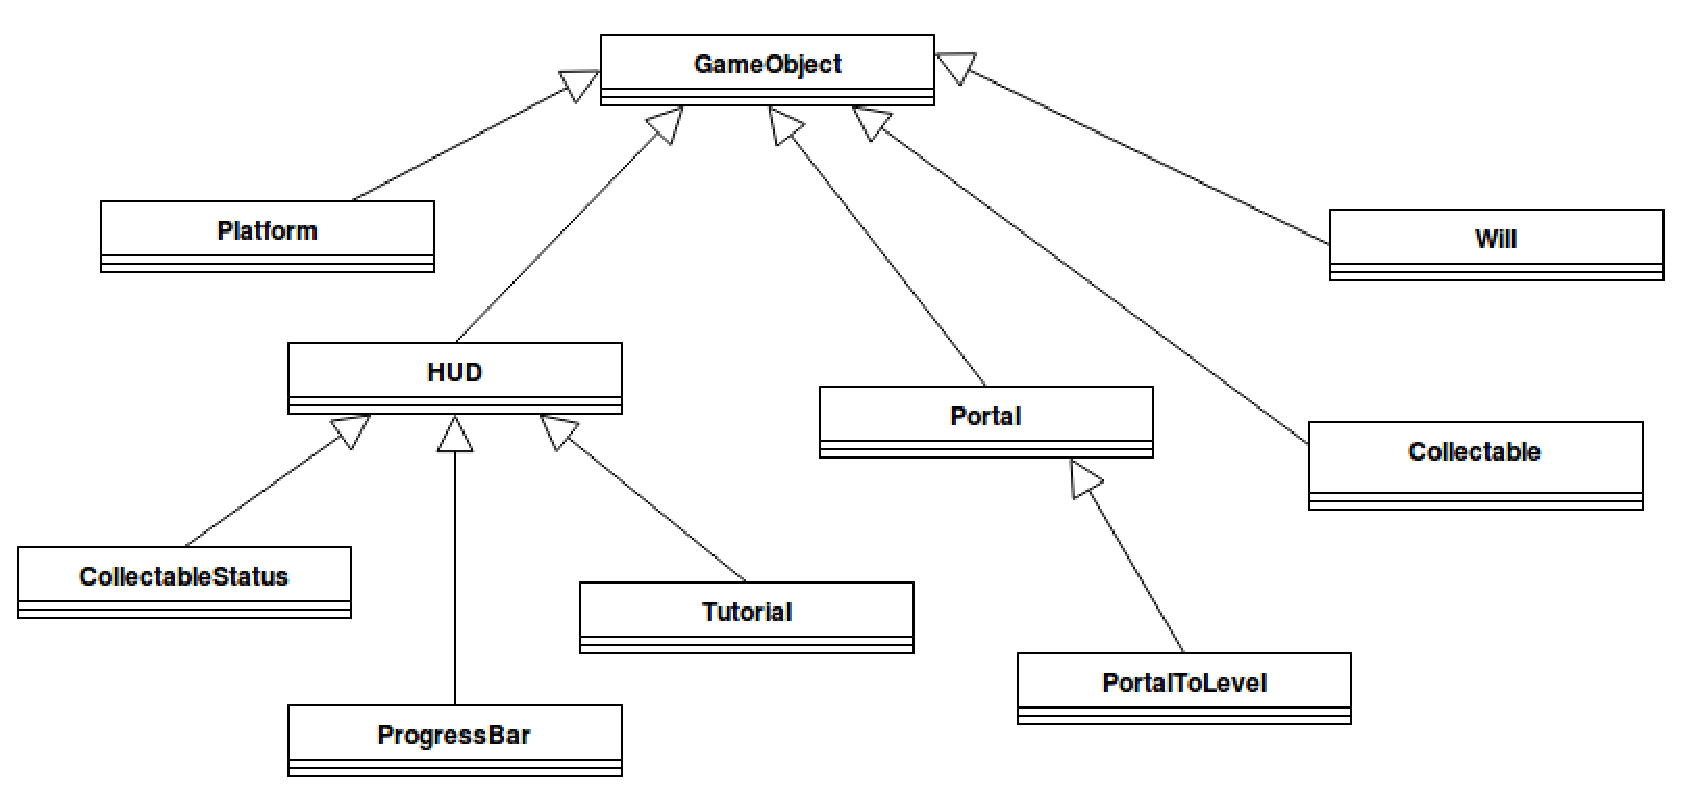
\includegraphics[keepaspectratio=true,scale=0.6]{figuras/class-diagram-1.eps}
        \caption[Modelagem inicial dos objetos do jogo]
          {Modelagem inicial dos objetos do jogo. Fonte: \textit{Autores}.}
        \label{game-object-children}
      \end{figure}

    \subsubsection{Níveis}

      A classe \textit{Level} contém a generalização de um nível no jogo. No jogo, os menus (principal e de seleção de fases), \textit{cutscenes}, fases e telas de vitória e derrota são representados como níveis do jogo.

      Abaixo se encontra a modelagem inicial dessas classes.

      \begin{figure}[H]
        \centering 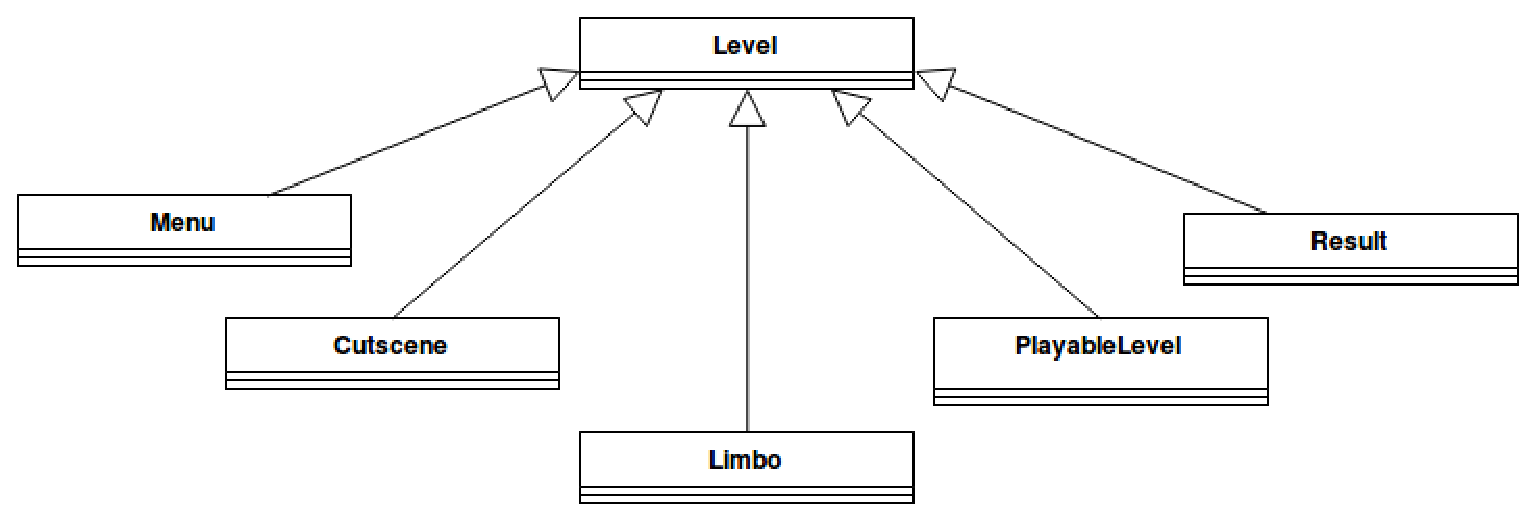
\includegraphics[keepaspectratio=true,scale=0.6]{figuras/class-diagram-2.eps}
        \caption[Modelagem inicial dos níveis do jogo]
          {Modelagem inicial dos níveis do jogo. Fonte: \textit{Autores}.}
        \label{game-object-levels}
      \end{figure}

    \subsubsection{Ajuste de recursos do jogo}

      Os recursos como imagens, áudios e arquivos de fonte do jogo precisarão ser editados para que possam ser carregados em memória e utilizados no GBA. No caso das imagens, por exemplo, serão modificadas características como dimensões e quantidade de cores a fim de diminuir seu tamanho para que possam ser convertidas para um formato utilizável no GBA.